\documentclass[10pt]{article}
\usepackage[english]{babel}
\usepackage{../../../meta-inf/lib/naproche}
\usepackage{amssymb}
\usepackage{mathtools} % for \coloneq

\usepackage{stex-highlighting}
\providebool{emph} % "\newbool{emph}" does not work...
\setbool{emph}{false}
\colorlet{emphcolor}{violet}
\let\oldemph\emph
\renewcommand\emph[1]{\setbool{emph}{true}\ifbool{forthel}{\textcolor{emphcolor}{\itshape#1}}{\oldemph{#1}}\setbool{emph}{false}}
\renewcommand{\varemph}[1]{\ifbool{emph}{\textcolor{emphcolor}{#1}}{\textcolor{black}{#1}}}

\usepackage[right=6cm,left=3cm,bottom=3cm,marginparwidth=5cm]{geometry}

\usepackage{fancyhdr}
\renewcommand{\sectionmark}[1]{\markboth{#1}{}} 
\def\libarchive{}
\pagestyle{fancy}
\fancyhead[L]{\libarchive}
\fancyhead[C]{\nouppercase\leftmark}  % section title
\fancyhead[R]{\thepage}               % page number
\fancyfoot[C]{}                       % No page number in footer

\usepackage[nobottomtitles]{titlesec}
\titlespacing*{\section}{0pt}{30pt}{0pt}
\titlespacing*{\subsection}{0pt}{30pt}{0pt}
\titlespacing*{\subsubsection}{0pt}{30pt}{0pt}

\documentclass[12pt,oneside]{book}

\usepackage[foundations]{../../lib/tex/naproche}
\usepackage{../../lib/tex/libraries}
\usepackage{graphicx}
\usepackage{float}
\usepackage{caption}
\usepackage{footnote}

\makesavenoteenv{tabular} % Make footnotes work in tabular environments


\title{Foundations of Mathematics}
\author{Marcel Schütz}
\date{2022}

\begin{document}
  \maketitle

  \tableofcontents

  \begin{figure}[H]
    \centering
    \fbox{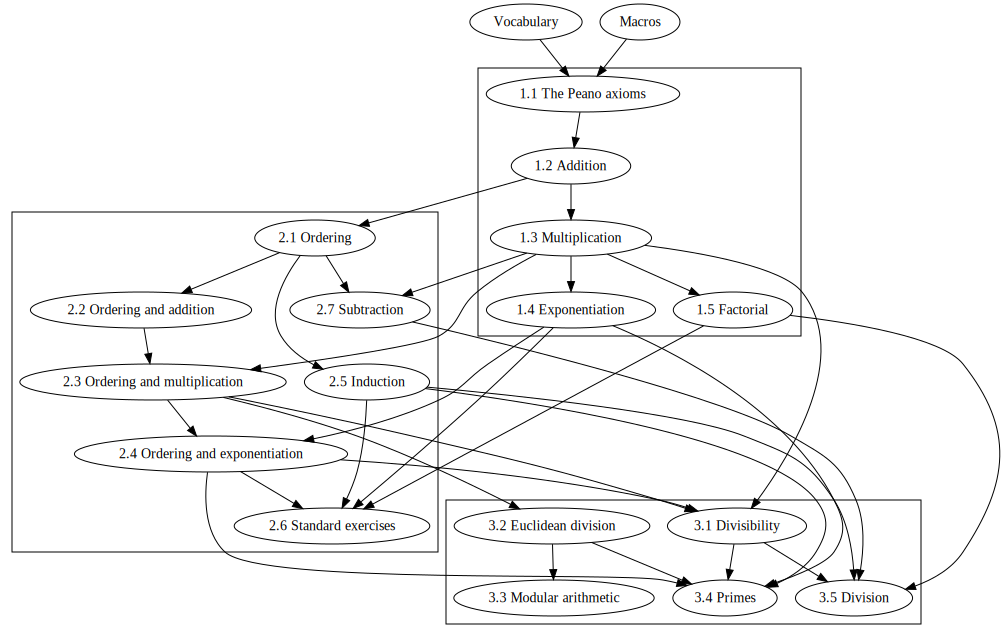
\includegraphics[width=0.9\linewidth]{./dependency-graph/graph.png}}
    \caption*{Interdependencies of the chapters}
  \end{figure}


  \section*{Introduction}

  This is a library providing a foundation of mathematics based on a
  Kelley-Morse like class theory with urelements.
  It introduces common operations on classes like unions or intersections
  (\cref{chapter:classes}) together with detailed proofs of their algebraic
  properties (\cref{chapter:computation-laws-for-classes}), the symmetric
  difference of two classes (\cref{chapter:symmetric-difference}) and the
  notions of ordered pairs and Cartesian products
  (\cref{chapter:pairs-and-products}) as well as proofs of the algebraic
  properties of the latter (\cref{chapter:computation-laws-for-products}).
  Moreover, it provides common operations on maps (\cref{chapter:maps}), various
  properties of images and preimages (\cref{chapter:image-and-preimage}) and the
  notions of injectivity, surjectivity, bijectivity
  (\cref{chapter:injections-surjections-bijections}) and invertibility of maps
  (\cref{chapter:invertible-maps}).
  The library provides an axiom system characterizing sets (\cref{chapter:sets})
  and, furthermore, it covers the notions of binary relations
  (\cref{chapter:binary-relations}), fixed-points of subset preserving maps
  (\cref{chapter:fixed-points}), including and equinumerosity
  (\cref{chapter:equinumerosity}).

  As two famous results it includes the Knaster-Tarski fixed point theorem
  (\cref{FOUNDATIONS_12_8420450166112256}) and the Cantor-Schröder-Bernstein
  theorem (\cref{FOUNDATIONS_13_1913663275401216}).

  \paragraph*{Usage.}
  At the very beginning of each chapter you can find the name of its source
  file, e.g. \path{foundations/sections/01_classes.ftl.tex} for
  \cref{chapter:classes}. This filename can be used to import the chapter via
  \Naproche's \texttt{readtex} instruction to another ForTheL text, e.g.:
  \begin{center}
    \verb`[readtex \path{foundations/sections/01_classes.ftl.tex}]`
  \end{center}

  \paragraph*{Checking times.}
  The checking times for each of the chapters may vary from computer to
  computer, but on mid-range hardware they are likely to be similar to those
  given in table below:

  \begin{center}
    \begin{tabular}{c|c|c}

      & \multicolumn{2}{c}{\textbf{Checking time}}
      \\
      \textbf{Chapter}
      & \textbf{without dependencies}     & \textbf{with dependencies}
      \\ \hline
      \ref{chapter:classes}
      & 00:04 min                         & 00:04 min
      \\
      \ref{chapter:computation-laws-for-classes}
      & 00:12 min                         & 00:16 min
      \\
      \ref{chapter:symmetric-difference}
      & 00:32 min                         & 00:48 min
      \\
      \ref{chapter:pairs-and-products}
      & 00:08 min                         & 00:12 min
      \\
      \ref{chapter:computation-laws-for-products}
      & 01:36 min                         & 01:56 min
      \\
      \ref{chapter:maps}
      & 01:13 min                         & 01:25 min
      \\
      \ref{chapter:image-and-preimage}
      & 01:28 min                         & 02:53 min
      \\
      \ref{chapter:injections-surjections-bijections}
      & 00:38 min                         & 02:03 min
      \\
      \ref{chapter:invertible-maps}
      & 02:20 min                         & 04:23 min
      \\
      \ref{chapter:sets}
      & 02:17 min                         & 06:40 min
      \\
      \ref{chapter:binary-relations}
      & 00:14 min                         & 06:54 min
      \\
      \ref{chapter:fixed-points}
      & 00:33 min                         & 07:13 min
      \\
      \ref{chapter:equinumerosity}
      & 01:48 min                         & 09:01 min
    \end{tabular}
  \end{center}


  \subfile{sections/01_classes.ftl.tex}
  \subfile{sections/02_computation-laws-for-classes.ftl.tex}
  \subfile{sections/03_symmetric-difference.ftl.tex}
  \subfile{sections/04_pairs-and-products.ftl.tex}
  \subfile{sections/05_computation-laws-for-products.ftl.tex}
  \subfile{sections/06_maps.ftl.tex}
  \subfile{sections/07_image-and-preimage.ftl.tex}
  \subfile{sections/08_injections-surjections-bijections.ftl.tex}
  \subfile{sections/09_invertible-maps.ftl.tex}
  \subfile{sections/10_sets.ftl.tex}
  \subfile{sections/11_binary-relations.ftl.tex}
  \subfile{sections/12_fixed-points.ftl.tex}
  \subfile{sections/13_equinumerosity.ftl.tex}
\end{document}

\begin{document}
  \begin{imports}
    \begin{forthel}
      %[prove off][check off]
      [readtex \path{libraries/source/foundations/classes.ftl.tex}]
      %[prove on][check on]
    \end{forthel}
  \end{imports}


  \section*{Computation Laws For Classes}

  \subsection*{Commutativity of Union and Intersection}

  \begin{forthel}
    \begin{proposition}[id=FOUNDATIONS_02_8446177632583680,printid]
      Let $A, B$ be classes.
      Then $A \cup B = B \cup A$.
    \end{proposition}
    \begin{proof}
      Let us show that $A \cup B \subseteq B \cup A$.
        Let $x \in A \cup B$.
        Then $x \in A$ or $x \in B$.
        Hence $x \in B$ or $x \in A$.
        Thus $x \in B \cup A$.
      End.

      Let us show that $B \cup A \subseteq A \cup B$.
        Let $x \in B \cup A$.
        Then $x \in B$ or $x \in A$.
        Hence $x \in A$ or $x \in B$.
        Thus $x \in A \cup B$.
      End.
    \end{proof}
  \end{forthel}

  \begin{forthel}
    \begin{proposition}[id=FOUNDATIONS_02_7565102251245568,printid]
      Let $A, B$ be classes.
      Then $A \cap B = B \cap A$.
    \end{proposition}
    \begin{proof}
      Let us show that $A \cap B \subseteq B \cap A$.
        Let $x \in A \cap B$.
        Then $x \in A$ and $x \in B$.
        Hence $x \in B$ and $x \in A$.
        Thus $x \in B \cap A$.
      End.

      Let us show that $B \cap A \subseteq A \cap B$.
        Let $x \in B \cap A$.
        Then $x \in B$ and $x \in A$.
        Hence $x \in A$ and $x \in B$.
        Thus $x \in A \cap B$.
      End.
    \end{proof}
  \end{forthel}


  \subsection*{Associativity of Union and Intersection}

  \begin{forthel}
    \begin{proposition}[id=FOUNDATIONS_02_3854032263184384,printid]
      Let $A, B, C$ be classes.
      Then $(A \cup B) \cup C = A \cup (B \cup C)$.
    \end{proposition}
    \begin{proof}
      Let us show that $((A \cup B) \cup C) \subseteq A \cup (B \cup C)$. %!
        Let $x \in (A \cup B) \cup C$.
        Then $x \in A \cup B$ or $x \in C$.
        Hence $x \in A$ or $x \in B$ or $x \in C$.
        Thus $x \in A$ or $x \in (B \cup C)$.
        Therefore $x \in A \cup (B \cup C)$.
      End.

      Let us show that $A \cup (B \cup C) \subseteq (A \cup B) \cup C$.
        Let $x \in A \cup (B \cup C)$.
        Then $x \in A$ or $x \in B \cup C$.
        Hence $x \in A$ or $x \in B$ or $x \in C$.
        Thus $x \in A \cup B$ or $x \in C$.
        Therefore $x \in (A \cup B) \cup C$.
      End.
    \end{proof}
  \end{forthel}

  \begin{forthel}
    \begin{proposition}[id=FOUNDATIONS_02_906751977193472,printid]
      Let $A, B, C$ be classes.
      Then $(A \cap B) \cap C = A \cap (B \cap C)$.
    \end{proposition}
    \begin{proof}
      Let us show that $((A \cap B) \cap C) \subseteq A \cap (B \cap C)$. %!
        Let $x \in (A \cap B) \cap C$.
        Then $x \in A \cap B$ and $x \in C$.
        Hence $x \in A$ and $x \in B$ and $x \in C$.
        Thus $x \in A$ and $x \in (B \cap C)$.
        Therefore$ x \in A \cap (B \cap C)$.
      End.

      Let us show that $A \cap (B \cap C) \subseteq (A \cap B) \cap C$.
        Let $x \in A \cap (B \cap C)$.
        Then $x \in A$ and $x \in B \cap C$.
        Hence $x \in A$ and $x \in B$ and $x \in C$.
        Thus $x \in A \cap B$ and $x \in C$.
        Therefore $x \in (A \cap B) \cap C$.
      End.
    \end{proof}
  \end{forthel}


  \subsection*{Distributivity of Union and Intersection}

  \begin{forthel}
    \begin{proposition}[id=FOUNDATIONS_02_371139087958016,printid]
      Let $A, B, C$ be classes.
      Then $A \cap (B \cup C) = (A \cap B) \cup (A \cap C)$.
    \end{proposition}
    \begin{proof}
      Let us show that $A \cap (B \cup C) \subseteq (A \cap B) \cup (A \cap C)$.
        Let $x \in A \cap (B \cup C)$.
        Then $x \in A$ and $x \in B \cup C$.
        Hence $x \in A$ and ($x \in B$ or $x \in C$).
        Thus ($x \in A$ and $x \in B$) or ($x \in A$ and $x \in C$).
        Therefore $x \in A \cap B$ or $x \in A \cap C$.
        Hence $x \in (A \cap B) \cup (A \cap C)$.
      End.

      Let us show that $((A \cap B) \cup (A \cap C)) \subseteq A \cap (B \cup C)$. %!
        Let $x \in (A \cap B) \cup (A \cap C)$.
        Then $x \in A \cap B$ or $x \in A \cap C$.
        Hence ($x \in A$ and $x \in B$) or ($x \in A$ and $x \in C$).
        Thus $x \in A$ and ($x \in B$ or $x \in C$).
        Therefore $x \in A$ and $x \in B \cup C$.
        Hence$ x \in A \cap (B \cup C)$.
      End.
    \end{proof}
  \end{forthel}

  \begin{forthel}
    \begin{proposition}[id=FOUNDATIONS_02_5937390721957888,printid]
      Let $A, B, C$ be classes.
      Then $A \cup (B \cap C) = (A \cup B) \cap (A \cup C)$.
    \end{proposition}
    \begin{proof}
      Let us show that $A \cup (B \cap C) \subseteq (A \cup B) \cap (A \cup C)$.
        Let $x \in A \cup (B \cap C)$.
        Then $x \in A$ or $x \in B \cap C$.
        Hence $x \in A$ or ($x \in B$ and $x \in C$).
        Thus ($x \in A$ or $x \in B$) and ($x \in$ A or $x \in C$).
        Therefore $x \in A \cup B$ and $x \in A \cup C$.
        Hence $x \in (A \cup B) \cap (A \cup C)$.
      End.

      Let us show that $((A \cup B) \cap (A \cup C)) \subseteq A \cup (B \cap C)$. %!
        Let $x \in (A \cup B) \cap (A \cup C)$.
        Then $x \in A \cup B$ and $x \in A \cup C$.
        Hence ($x \in A$ or $x \in B$) and ($x \in A$ or $x \in C$).
        Thus $x \in A$ or ($x \in B$ and $x \in C$).
        Therefore $x \in A$ or $x \in B \cap C$.
        Hence $x \in A \cup (B \cap C)$.
      End.
    \end{proof}
  \end{forthel}


  \subsection*{Idempocy Laws for Union and Intersection}

  \begin{forthel}
    \begin{proposition}[id=FOUNDATIONS_02_2096996737351680,printid]
      Let $A$ be a class.
      Then $A \cup A = A$.
    \end{proposition}
    \begin{proof}
      $A \cup A = \{x \mid x \in A$ or $x \in A \}$.
      Hence $A \cup A = \{ x \mid x \in A \}$.
      Thus $A \cup A = A$.
    \end{proof}
  \end{forthel}

  \begin{forthel}
    \begin{proposition}[id=FOUNDATIONS_02_4053144145231872,printid]
      Let $A$ be a class.
      Then $A \cap A = A$.
    \end{proposition}
    \begin{proof}
      $A \cap A = \{ x \mid x \in A$ and $x \in A \}$.
      Hence $A \cap A = \{ x \mid x \in A \}$.
      Thus $A \cap A = A$.
    \end{proof}
  \end{forthel}


  \subsection*{Distributivity of Complement}

  \begin{forthel}
    \begin{proposition}[id=FOUNDATIONS_02_5296031436636160,printid]
      Let $A, B, C$ be classes.
      Then $A \setminus (B \cap C) = (A \setminus B) \cup (A \setminus C)$.
    \end{proposition}
    \begin{proof}
      Let us show that $A \setminus (B \cap C) \subseteq (A \setminus B) \cup (A \setminus C)$.
        Let $x \in A \setminus (B \cap C)$.
        Then $x \in A$ and $x \notin B \cap C$.
        Hence it is wrong that ($x \in B$ and $x \in C$).
        Thus $x \notin B$ or $x \notin C$.
        Therefore $x \in A$ and ($x \notin B$ or $x \notin C$).
        Then ($x \in A$ and $x \notin B$) or ($x \in A$ and $x \notin C$).
        Hence $x \in A \setminus B$ or $x \in A \setminus C$.
        Thus $x \in (A \setminus B) \cup (A \setminus C)$.
      End.

      Let us show that $((A \setminus B) \cup (A \setminus C)) \subseteq A \setminus (B \cap C)$. %!
        Let $x \in (A \setminus B) \cup (A \setminus C)$.
        Then $x \in A \setminus B$ or $x \in A \setminus C$.
        Hence ($x \in A$ and $x \notin B$) or ($x \in A$ and $x \notin C$).
        Thus $x \in A$ and ($x \notin B$ or $x \notin C$).
        Therefore $x \in A$ and not ($x \in B$ and $x \in C$).
        Then $x \in A$ and not $x \in B \cap C$.
        Hence $x \in A \setminus (B \cap C)$.
      End.
    \end{proof}
  \end{forthel}

  \begin{forthel}
    \begin{proposition}[id=FOUNDATIONS_02_2909554153095168,printid]
      Let $A, B, C$ be classes.
      Then $A \setminus (B \cup C) = (A \setminus B) \cap (A \setminus C)$.
    \end{proposition}
    \begin{proof}
      Let us show that $A \setminus (B \cup C) \subseteq (A \setminus B) \cap (A \setminus C)$.
        Let $x \in A \setminus (B \cup C)$.
        Then $x \in A$ and $x \notin B \cup C$.
        Hence it is wrong that ($x \in B$ or $x \in C$).
        Thus $x \notin B$ and $x \notin C$.
        Therefore $x \in A$ and ($x \notin B$ and $x \notin C$).
        Then ($x \in A$ and $x \notin B$) and ($x \in A$ and $x \notin C$).
        Hence $x \in A \setminus B$ and $x \in A \setminus C$.
        Thus $x \in (A \setminus B) \cap (A \setminus C)$.
      End.

      Let us show that $((A \setminus B) \cap (A \setminus C)) \subseteq A \setminus (B \cup C)$. %!
        Let $x \in (A \setminus B) \cap (A \setminus C)$.
        Then $x \in A \setminus B$ and $x \in A \setminus C$.
        Hence ($x \in A$ and $x \notin B$) and ($x \in A$ and $x \notin C$).
        Thus $x \in A$ and ($x \notin B$ and $x \notin C$).
        Therefore $x \in A$ and not ($x \in B$ or $x \in C$).
        Then $x \in A$ and not $x \in B \cup C$.
        Hence $x \in A \setminus (B \cup C)$.
      End.
    \end{proof}
  \end{forthel}


  \subsection*{Subclass Laws}

  \begin{forthel}
    \begin{proposition}[id=FOUNDATIONS_02_3793981508943872,printid]
      Let $A, B$ be classes.
      Then $A \subseteq A \cup B$.
    \end{proposition}
    \begin{proof}
      Let $x \in A$.
      Then $x \in A$ or $x \in B$.
      Hence $x \in A \cup B$.
    \end{proof}
  \end{forthel}

  \begin{forthel}
    \begin{proposition}[id=FOUNDATIONS_02_1591517646946304,printid]
      Let $A, B$ be classes.
      Then $A \cap B \subseteq A$.
    \end{proposition}
    \begin{proof}
      Let $x \in A \cap B$.
      Then $x \in A$ and $x \in B$.
      Hence $x \in A$.
    \end{proof}
  \end{forthel}

  \begin{forthel}
    \begin{proposition}[id=FOUNDATIONS_02_6657236858306560,printid]
      Let $A, B$ be classes.
      Then $A \subseteq B$ iff $A \cup B = B$.
    \end{proposition}
    \begin{proof}
      Case $A \subseteq B$.

        Let us show that $A \cup B \subseteq B$.
          Let $x \in A \cup B$.
          Then $x \in A$ or $x \in B$.
          If $x \in A$ then $x \in B$.
          Hence $x \in B$.
        End.

        Let us show that $B \subseteq A \cup B$.
          Let $x \in B$.
          Then $x \in A$ or $x \in B$.
          Hence $x \in A \cup B$.
        End.
      End.

      Case $A \cup B = B$.
        Let $x \in A$.
        Then $x \in A$ or $x \in B$.
        Hence $x \in A \cup B = B$.
      End.
    \end{proof}
  \end{forthel}

  \begin{forthel}
    \begin{proposition}[id=FOUNDATIONS_02_2356449346846720,printid]
      Let $A, B$ be classes.
      Then $A \subseteq B$ iff $A \cap B = A$.
    \end{proposition}
    \begin{proof}
      Case $A \subseteq B$.

        Let us show that $A \cap B \subseteq A$.
          Let $x \in A \cap B$.
          Then $x \in A$ and $x \in B$.
          Hence $x \in A$.
        End.

        Let us show that $A \subseteq A \cap B$.
          Let $x \in A$.
          Then $x \in B$.
          Hence $x \in A$ and $x \in B$.
          Thus $x \in A \cap B$.
        End.
      End.

      Case $A \cap B = A$.
        Let $x \in A$.
        Then $x \in A \cap B$.
        Hence $x \in A$ and $x \in B$.
        Thus $x \in B$.
      End.
    \end{proof}
  \end{forthel}


  \subsection*{Complement Laws}

  \begin{forthel}
    \begin{proposition}[id=FOUNDATIONS_02_7433299337150464,printid]
      Let $A$ be a class.
      Then $A \setminus A = \emptyset$.
    \end{proposition}
    \begin{proof}
      $A \setminus A$ has no elements.
      Indeed $A \setminus A = \{ x \mid x \in A$ and $x \notin A \}$.
      Hence the thesis.
    \end{proof}
  \end{forthel}

  \begin{forthel}
    \begin{proposition}[id=FOUNDATIONS_02_3783696985358336,printid]
      Let $A$ be a class.
      Then $A \setminus \emptyset = A$.
    \end{proposition}
    \begin{proof}
      $A \setminus \emptyset = \{ x \mid x \in A$ and $x \notin \emptyset \}$.
      No element is an element of $\emptyset$.
      Hence $A \setminus \emptyset = \{ x \mid x \in A \}$.
      Then we have the thesis.
    \end{proof}
  \end{forthel}

  \begin{forthel}
    \begin{proposition}[id=FOUNDATIONS_02_7083929257377792,printid]
      Let $A, B$ be classes.
      Then $A \setminus (A \setminus B) = A \cap B$.
    \end{proposition}
    \begin{proof}
      Let us show that $A \setminus (A \setminus B) \subseteq A \cap B$.
        Let $x \in A \setminus (A \setminus B)$.
        Then $x \in A$ and $x \notin A \setminus B$.
        Hence $x \notin A$ or $x \in B$.
        Thus $x \in B$.
        Therefore $x \in A \cap B$.
      End.

      Let us show that $A \cap B \subseteq A \setminus (A \setminus B)$.
        Let $x \in A \cap B$.
        Then $x \in A$ and $x \in B$.
        Hence $x \notin A$ or $x \in B$.
        Thus $x \notin A \setminus B$.
        Therefore $x \in A \setminus (A \setminus B)$.
      End.
    \end{proof}
  \end{forthel}

  \begin{forthel}
    \begin{proposition}[id=FOUNDATIONS_02_4938646769631232,printid]
      Let $A, B$ be classes.
      Then $B \subseteq A$ iff $A \setminus (A \setminus B) = B$.
    \end{proposition}
    \begin{proof}
      Case $B \subseteq A$. Obvious.

      Case $A \setminus (A \setminus B) = B$.
        Then every element of $B$ is an element of $A \setminus (A \setminus B)$.
        Thus every element of $B$ is an element of $A$.
        Then we have the thesis.
      End.
    \end{proof}
  \end{forthel}

  \begin{forthel}
    \begin{proposition}[id=FOUNDATIONS_02_5811954316738560,printid]
      Let $A, B, C$ be classes.
      Then $A \cap (B \setminus C) = (A \cap B) \setminus (A \cap C)$.
    \end{proposition}
    \begin{proof}
      Let us show that $A \cap (B \setminus C) \subseteq (A \cap B) \setminus (A \cap C)$.
        Let $x \in A \cap (B \setminus C)$.
        Then $x \in A$ and $x \in B \setminus C$.
        Hence $x \in A$ and $x \in B$.
        Thus $x \in A \cap B$ and $x \notin C$.
        Therefore $x \notin A \cap C$.
        Then we have $x \in (A \cap B) \setminus (A \cap C)$.
      End.

      Let us show that $((A \cap B) \setminus (A \cap C)) \subseteq A \cap (B \setminus C)$. %!
        Let $x \in (A \cap B) \setminus (A \cap C)$.
        Then $x \in A$ and $x \in B$.
        $x \notin A \cap C$.
        Hence $x \notin C$.
        Thus $x \in B \setminus C$.
        Therefore $x \in A \cap (B \setminus C)$.
      End.
    \end{proof}
  \end{forthel}
\end{document}
